\section{Evaluation}
\label{sec:eval}

In this section we present a qualitative evaluation that compares Flow and the NDN-IoT framework with the conceptual implementations of a similar gaming system over AWS IoT and Apple HomeKit (using TCP/IP architecture).
The goal of this side-by-side comparison is to highlight the differences between the proposed architecture and the current practice in the industry, and point out how the NDN architecture simplifies the design and implementation of a cloud-independent IoT system.
Fig.~\ref{fig:compare-ecosystems} shows three different designs of home entertainment system over AWS IoT, Apple HomeKit, and NDN-IoT, respectively.

\begin{figure*}[!t]
\centering
\subfloat[Conceptual system over AWS IoT]{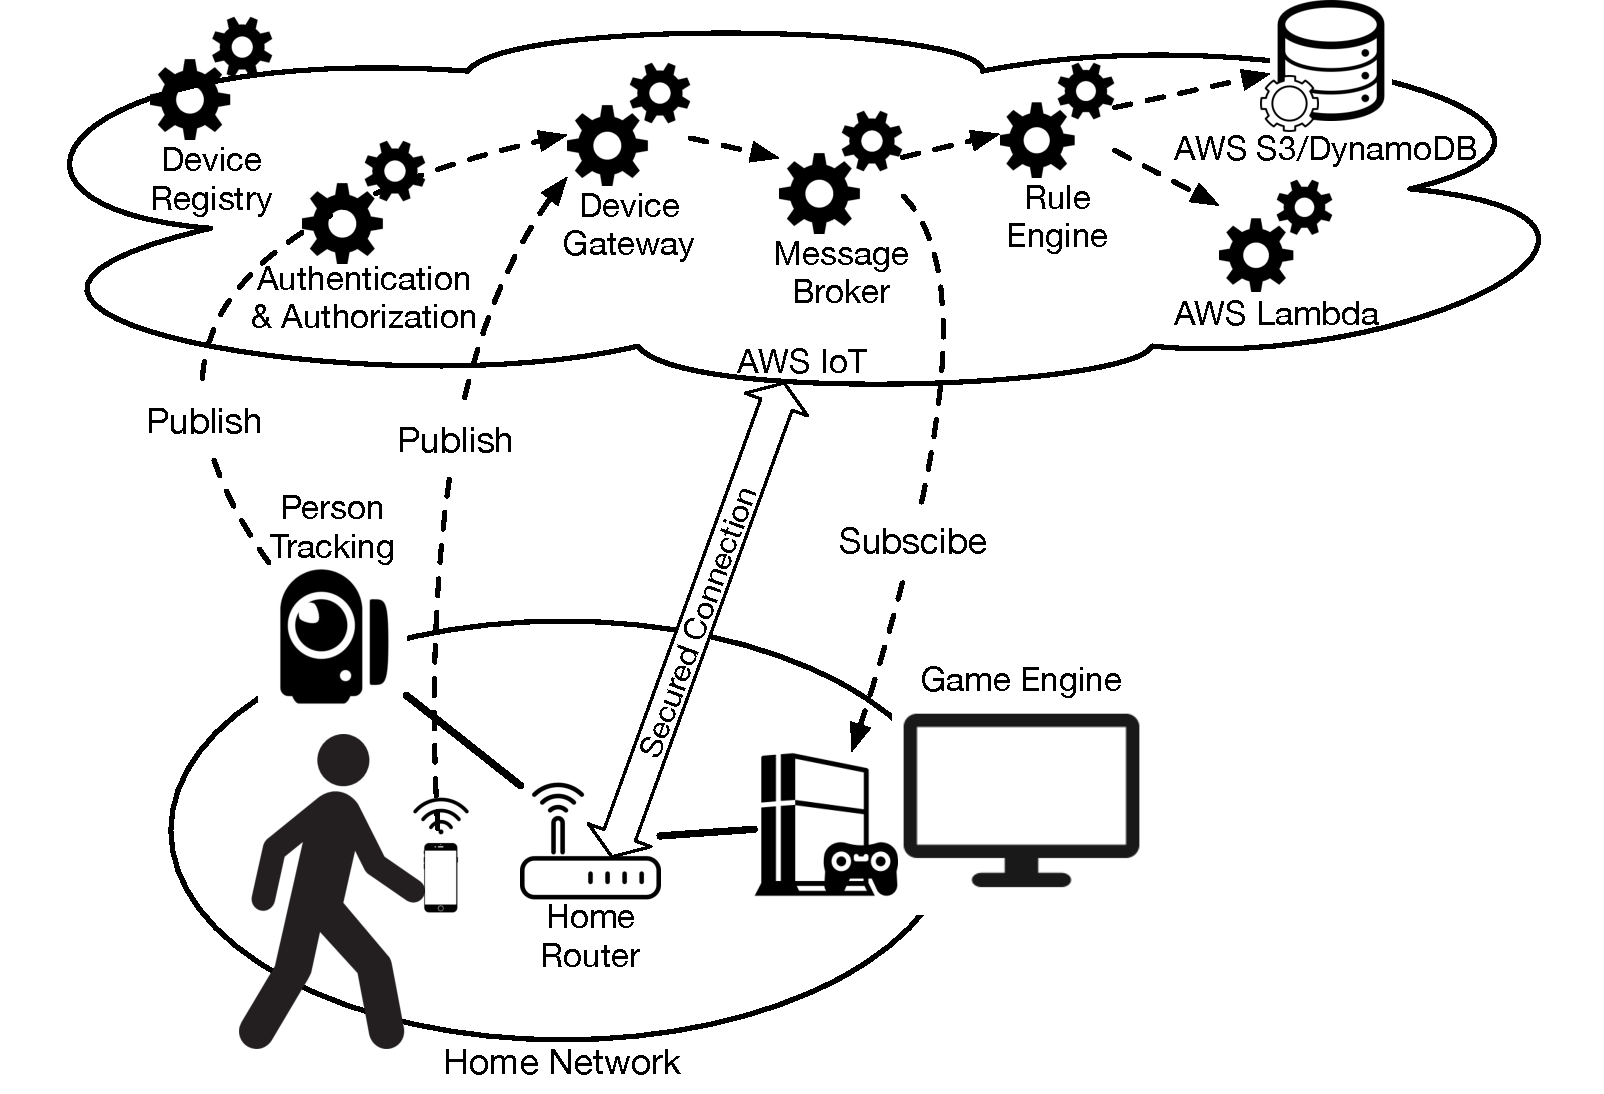
\includegraphics[width=0.37\textwidth]{aws-concept.pdf}%
\label{fig:aws-concept}}
\hfil
\subfloat[Conceptual system over HomeKit]{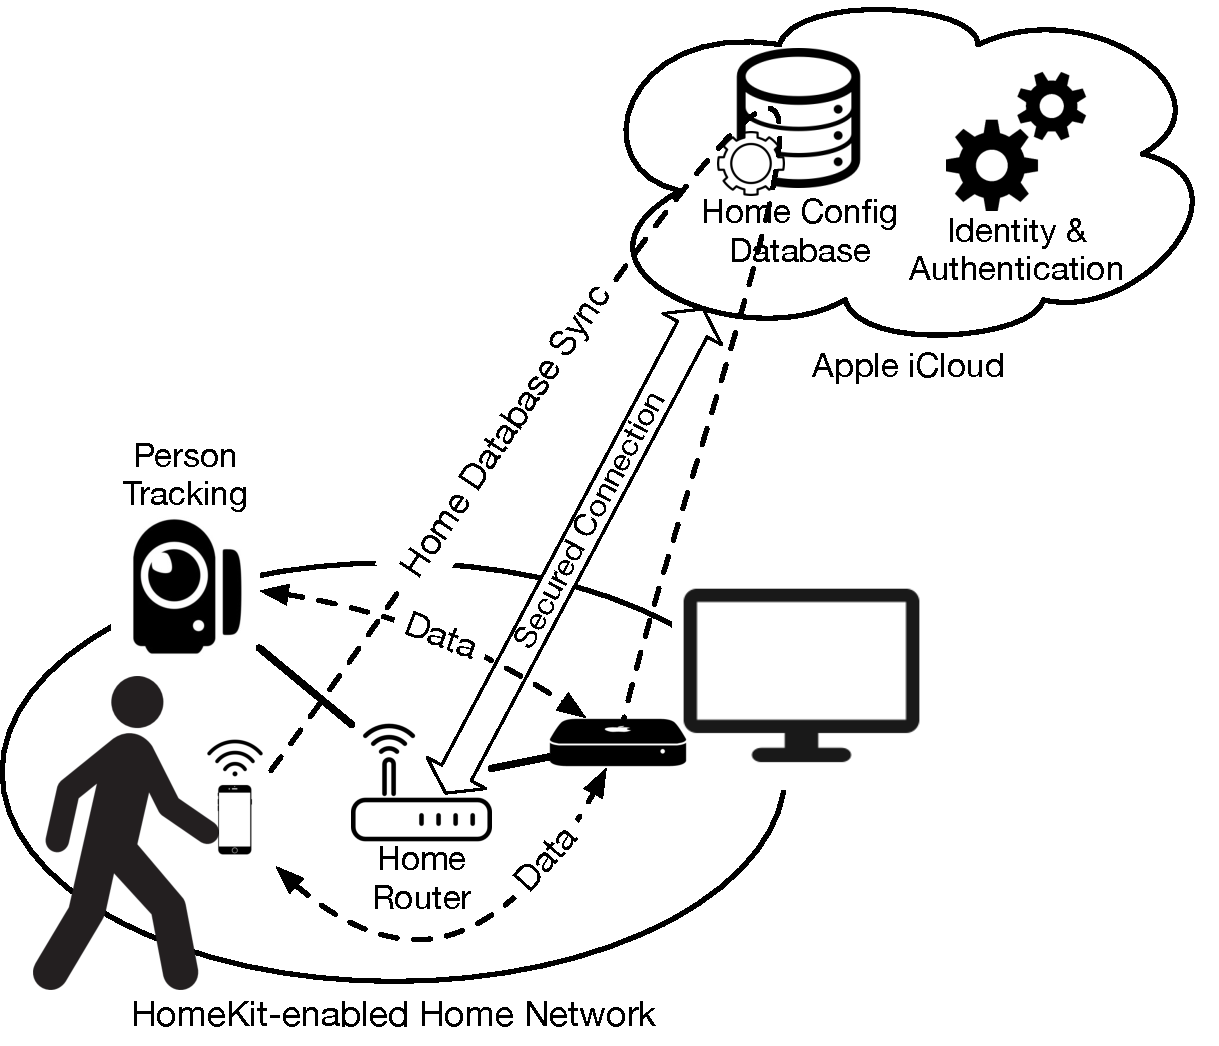
\includegraphics[width=0.3\textwidth]{homekit-concept.pdf}%
\label{fig:homekit-concept}}
\hfil
\subfloat[Actual implementation over NDN-IoT]{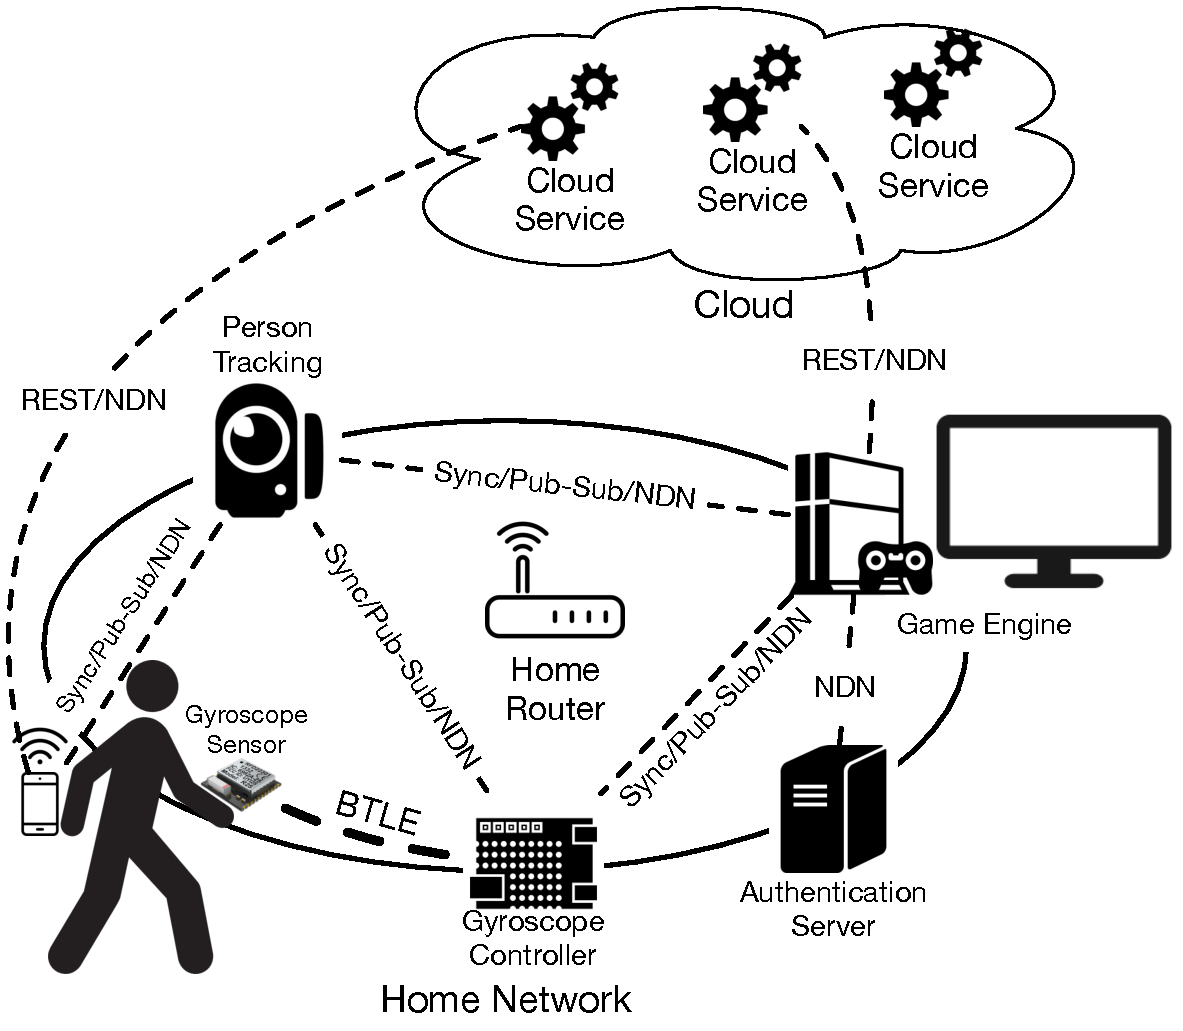
\includegraphics[width=0.3\textwidth]{flow-ndn-iot.pdf}%
\label{fig:flow-ndn-iot}}
\caption{Comparison of IoT-enabled home entertainment systems over different ecosystems.}
\label{fig:compare-ecosystems}
\end{figure*}

In Fig.~\ref{fig:aws-concept}, all local devices are certified by the AWS IoT Registry service in order to join the IoT system.
Application data generated by the person tracking device and the user smartphone need to go through the pub-sub message brokers (e.g., via MQTT) in the cloud who will route the messages to the game engine back in the local network or AWS services in the cloud according user-defined rules.
There is a significant amount of work performed by the AWS infrastructure to map user-defined device names to the underlying TLS tunnels, maintain soft-state about device configuration and latest status, manage the pub-sub channels between data producers and consumers, and enforce authentication and access control policies during message exchange.

Being the least cloud-dependent among the existing IoT ecosystems, HomeKit reduces the dependency on the cloud to two key services only:
providing and authenticating the identities of devices and users during the bootstrap phase, and synchronizing the home configuration database across multiple devices.
The game engine device in Fig.~\ref{fig:homekit-concept} can look up in its local copy of that database to discover the person tracking device and gyroscope sensor in the same local network.
There is a separate auto-configuration process based on mDNS to discover network addresses and set up direct TCP/IP connections among devices over local Wi-Fi or Ethernet.

Without requiring cloud connectivity, the NDN-IoT framework covers most of the services shown in Fig.~\ref{fig:service-arch}, with access control left as future work.\footnote{We expect to apply previous work in~\cite{nac}.}
In Flow/NDN-IoT (shown in Fig.~\ref{fig:flow-ndn-iot}), rendezvous and discovery built on top of a decentralized synchronization protocol allows the game engine to find the person tracking device and gyroscope sensors in the local network automatically;
the trust schema rooted at the local trust anchor allows the game engine to authenticate the data produced by other devices without establishing secured tunnels to either the local devices or the remote cloud;
application data messaging is efficiently supported by the NDN network layer protocol for both local and remote access, without requiring additional services to configure network addresses or resolve names to addresses;
cloud services become an optional component that facilitates, rather than dictates, the local IoT functions.
